\documentclass[a4paper, 11pt]{scrartcl}

%% Language and font encodings
\usepackage[english]{babel}
\usepackage[utf8x]{inputenc}


%% Sets page size and margins
\usepackage[a4paper,top=3cm,bottom=2cm,left=3cm,right=3cm,marginparwidth=1.75cm]{geometry}

%% Useful packages
\usepackage{amsmath}
\usepackage{graphicx}
\usepackage{float}
\usepackage{url}
\usepackage{listings}
\usepackage[colorinlistoftodos]{todonotes}
\usepackage[colorlinks=true, allcolors=blue]{hyperref}

\usepackage{authblk}

\lstdefinelanguage{F}{%
	language     = C,
	morekeywords = {fract},
	basicstyle=\ttfamily,
	keywordstyle=\color{blue}\ttfamily,
	stringstyle=\color{red}\ttfamily,
	commentstyle=\color{gray}\ttfamily,
	morecomment=[l][\color{magenta}]{\#}
}

\title{FAC - F Academic Compiler}
\author[1]{Mirko Bez}
\author[2]{Stefano Munari}
\affil[1]{\href{mailto:mirko.bez@studenti.unipd.it}{mirko.bez@studenti.unipd.it}}
\affil[2]{\href{mailto:stefano.munari.1@studenti.unipd.it}{stefano.munari.1@studenti.unipd.it}}

% Image directory
\graphicspath{{res/img/}}
% Set path for the sections
\makeatletter
\providecommand*{\input@path}{}
\g@addto@macro\input@path{{section/}}% append
\makeatother


\begin{document}
\maketitle
\tableofcontents
\listoffigures
\lstlistoflistings
\newpage
\section*{Introduction}

FAC is the front end part of a compiler which translates programs written in the
F language into a target representation. FAC is written in C using
flex \cite{flex-online} and bison \cite{bison-online}.
It is interesting to note that FAC can potentially support many target
representations.

\subsection*{Architecture}
Fig. \ref{fig:arch-ovw} describes the architecture of FAC.
Its high-level structure is formed by two macro components:
\begin{itemize}
\item Lexer - the lexical analyzer;
\item Parser - which is divided into three parts:
\begin{itemize}
	\item Syntax analysis;
	\item Static semantic analysis;
	\item Target code generation.
\end{itemize}
\end{itemize}

FAC has been written to be modular. Indeed, it is possible to translate any F
program into other representations simply by writing a new printer implementation.
\\
In FAC a printer is a component which takes the three address code (3AC) of an F
program given as input and generates a version of that code translated into a targeted
representation.
\\
Currently, FAC supports three printers:
\begin{itemize}
\item IR (Internal Representation) - useful for educational purposes or to quickly debug the 3AC;
\item C - prints a C program;
\item Java\footnote{for time reasons only the skeleton has been implemented} - prints a Java program.
\end{itemize}

We chose to use two different intermediate representations:
\begin{itemize}
\item Abstract Syntax Three (AST) - because it is easy to perform semantic analysis on this structure;
\item Three Address Code (3AC) - because it is easy to perform code generation by parsing this structure.
\end{itemize}

\begin{figure}[H]
  \centering
  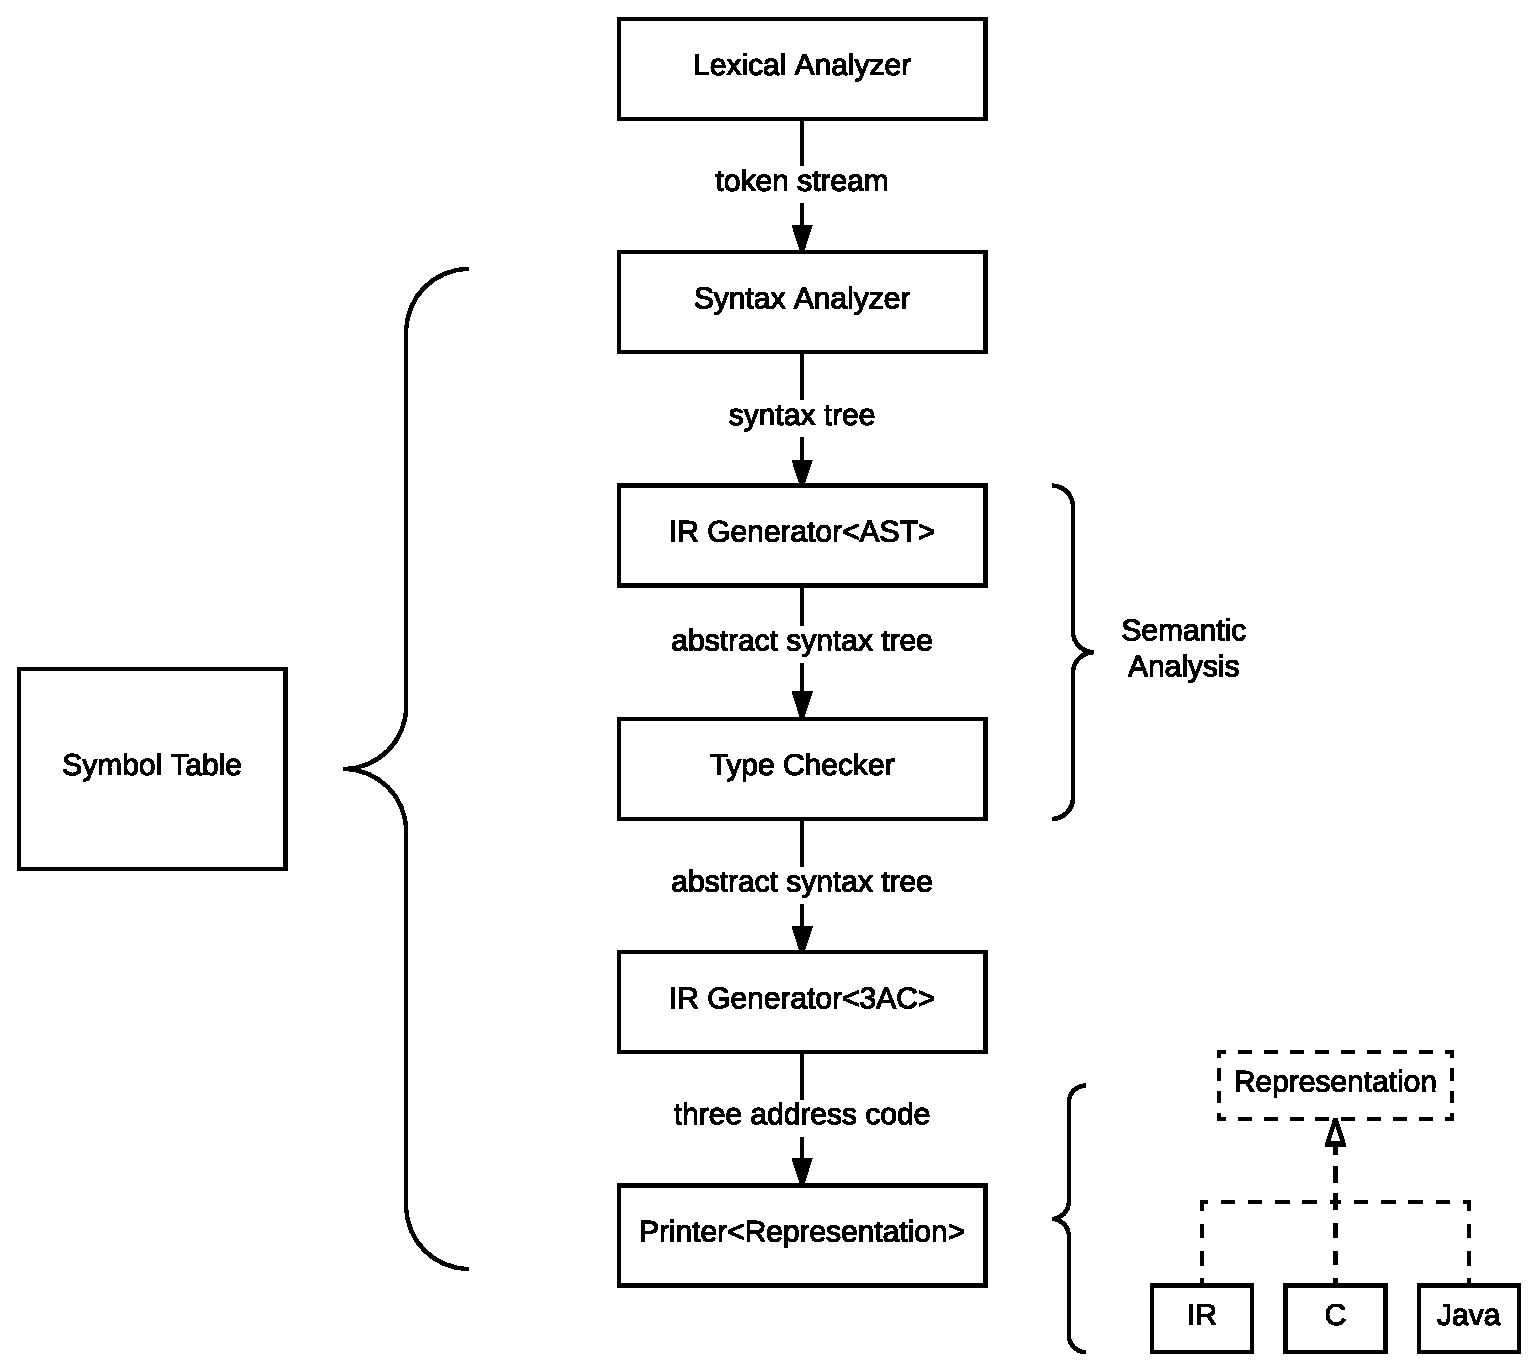
\includegraphics[width=.9\columnwidth]{img/eps/architecture.eps}
  \caption{Architectural Overview of the FAC compiler.}
  \label{fig:arch-ovw}
\end{figure}

\section{Lexer}
The lexical analyzer has been written using flex.
It has the following responsabilities:
\begin{itemize}
\item Verify that the input stream is lexically correct;
\item Produce the token stream for the parser;
\item Set the \verb|bison/flex| variable \verb|yylloc| -- this
variable contains the information about the first column, last column,
first row and last row of the token read. More details on its usage in
bison can be read in section \ref{sec:parser}.
\item Raise an error in case of a fract constant with denominator equal
to $0$ -- it is simply not considered as a valid lexeme.
\end{itemize}

\subsection{Lexemes}
We chose to define an identifier for each lexem, this enable us to change the
syntax of the F language without affecting its semantics and the other
components. Basically, the goal of this choice is to have something similar to
a C macro or a placeholder for the syntax symbols of the F language.
For example we have defined \verb|SUM| which is a placeholder for \verb|+|, so
if tomorrow we decide to use \verb|plus| to perform the arithmetic sum we can do
it transparently to the rest of the FAC code. This provides a great flexibility
for lexer symbols.

\subsection{Comments}
We have also implemented the regex which checks the comments. So it is possible
to write comments in the source code of F programs. They will be simply 
discarded during the phase of lexical analysis.

\subsection{Options}
We have used some flex options which enable optimizations
and to track the source code lines during the lexical analysis. Indeed, the
generated lexer does not contain a compressed table but a larger one which can
be accessed faster than the compressed one. Also, we used the align option to
notify flex to align memory access location of the generated table when
possible. Unfortunately, the line tracking option kills the performances.
In this case we have opted for a cleaner solution than an efficient one.

\subsection{Modularity}
The lexer can be generated on the fly. Indeed, each regex and each rule are
contained in a file which reflects respectively the regex and the rule purpose.
The regexs and the rules are automatically assembled by a Python script.
The script reads two configuration files written in json. These files specify
the order in which the regexs and the rules have to be written in the
\path{lexer.fl} file. Thus we can simply modify the configuration files to 
change the precedence of the lexer rules\footnote{Precedence rules are 
applied only in case of a tie.}.

\section{Parser}
\label{sec:parser}
The main goal of the parser written in bison is to check the
syntax correctness and to produce the Abstract Syntax Tree (AST).

\subsection{F -- Syntax choices}
We think that a language for students of the middle-school,
who are neophyte programmers, should be statically typed and type safe. 
At the same time it should be easy to use. 
Indeed, these requirements can help the student to learn how a simple 
high-level language works by discriminating between the different types.
In particular our minimal type system provides two completely unrelated types.
introduce some syntactic sugar, e.g. we 
provide directly the implication operator between boolean expression.

Thus we discriminated these types by introducing specific boolean
operators (in addition to the one usually provided):
\begin{itemize}
	\item \verb|XOR| - exclusive or;
	\item \verb|<->| - logical biimplication (syntactic sugar);
	\item \verb|->| - logical implication (syntactic sugar);
\end{itemize}

The rest is very similar to the C one. There is only a slight difference
for the arithmetic disequality. We preferred the Pascal \verb|<>| over 
the C \verb|!=|.

The syntactic symbols exist \emph{only} in the lexer. In the
rest of the program, i.e. in the parser and in the semantic analyser, only
internal representation of the operators are used. Therefore each grammar
symbol can be safely replaced without affecting the correctness of FAC.


\section{Symbol Table}
The symbol table has been implemented using
\href{https://troydhanson.github.io/uthash/}{uthash} because it is a reliable
and efficient solution to implement a symbol table.
\\
Basically, the symbol table contains the variables used in the program.
For each variable the symbol table stores:
\begin{itemize}
	\item the identifier;
	\item the type;
	\item value.
\end{itemize}

The symbol table is fundamental during the type checking and also during the
code generation phase. During the first phase it provides the type to the
type checker while during the second phase it provides also the value.
\section{Type-Checking}
\label{sec:type-checking}

The type-checker receives as input the AST created by the 
parser. This data structure is convenient to perform
type checking because it gets rid of the syntactic symbols and also because it 
is easily traversable.
In our implementation each operator is wrapped into a category.
For instance the operators \verb|LT, LE, EQ, NEQ, GT, GE| belongs to the 
category \verb|RELOP|. So, we need only a single type system rule for all the
operations of the same category.
This makes the implementation of the type checker more maintainable.


As already mentioned, in our implementation we distinguish between two types:
boolean and fract. Each time a variable is declared its type is saved into the 
corresponding symbol table entry, thus facilitating the type checking.

So, we implemented a simple type system which exploits the symbol
table as the context. Each time a new variable is declared 
the context is updated with the new variable. This allows us to find whenever
a variable is used before its declaration.

\section{Three Address Code}
We have implemented the three address code (3AC) using indirect triples. 
As stated by Aho et al. \cite{dragonbook}, this 
representation can help during the code optimization phase.
Indeed, the code optimizer can easily reorder the instructions without affecting
the triples themselves.

We generated the 3AC from the AST filtered by the type checker. 
To make it even easier to deal the instructions we chose to use
doubly-linked lists.

The following F code is represented in 3AC as depicted in Fig. 
\ref{fig:ind-trpl}:
\begin{verbatim}
fract a = [1|1];
fract b = [1|3] * a + [1|2];
\end{verbatim}

While traversing the AST we generate the three address code in a bottom up
fashion using \emph{only} synthesized attributes. This makes the three address
code generator intuitive.

\begin{figure}[H]
  \centering
  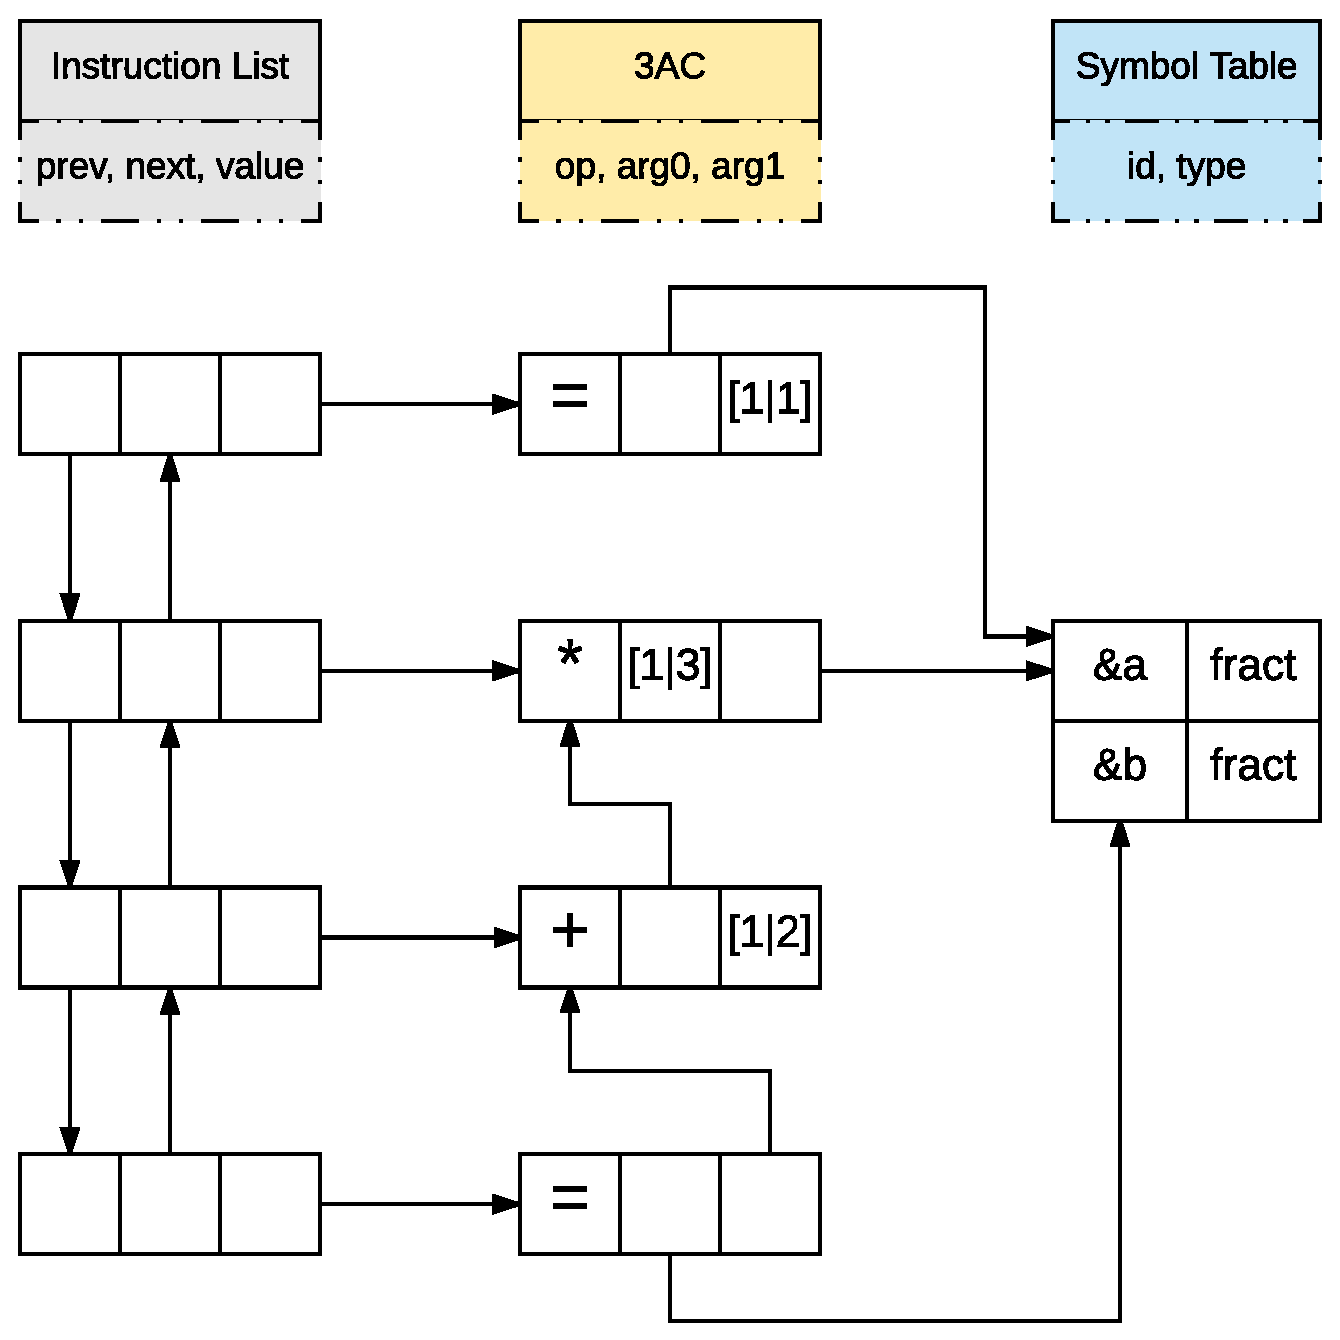
\includegraphics[width=.9\columnwidth]{img/eps/indirect_triples.eps}
  \caption{FAC - example of indirected triples.}
  \label{fig:ind-trpl}
\end{figure}

\section{Target Code Generator}

In FAC, the target code generator (aka printer) takes the
three address code (3AC) of an F program given as input and generates a version
of this code translated into a targeted representation.
\\
We have implemented the printer by constructing a virtual table
(using structs) which enables us to apply dynamic dispatching based on the
specific type of the printer. Basically, we copied the idea applied by the C++
compiler (over simplifying it) to implement dynamic dispatching on the top of C.
\\
Currently, FAC supports three printers:
\begin{itemize}
\item IR (Internal Representation) -- useful for educational purposes or to
quickly debug the 3AC;
\item C -- prints a C program;
\item Java\footnote{For time reasons only the skeleton has been implemented.}
-- prints a Java program.
\end{itemize}

The rational behind this choice is the extensibility. Indeed in the future
FAC could be extended even with target machine specific printers.


\section{Conclusion}
\subsection{Difficulties encountered}
The implementation of the 3AC generator along with the C printer implementation 
(these components are related) have been the hardest part of the project. The 
difficulty was mostly due the lack of a clear track to proceed. Indeed, we
had to choose how to build the 3AC specific implementation. Initially we tried
to implement a recursive version of the generator by passing the partial 3AC 
list to the successors and delegating the completion of a subtree 
(concatenating one or more lists) to the leaves. However, this approach was soon 
discarded because too complicated to implement. So, we decide to implement a 
recursive 3AC generator a bit more inefficient but a lot more clear and simple. 
Basically, the lists of the 3AC are constructed when returning from the 
recursive invocations and each composite case (e.g. if-then-else, assignment, 
etc.) handles its subtree (lists) connections.
\subsection{Future works}
\paragraph{Design}
To improve the current FAC front end design we think that a stronger decoupling 
of the components is necessary. The interfaces and their relationships are of 
fundamental importance for the development of the system. Currently, the code 
suffers from the god class anti pattern \cite{Martin:2008:CCH:1388398}. 
The parser concentrates too much dependencies and responsibilities inside 
itself. All the invocations to the AST generator, the type checker, the 3AC 
generator and the printer are performed by the parser! This problem was due to a
short-sighted design decision taken when we started building the parser. 
Unfortunately, proceeding with the project, we did not find the time to refactor 
this component (the parser). Indeed, other components needed to be implemented 
in time to complete the project and to do not miss the deadline.

\paragraph{Features}
Other interesting features that could be implemented are:
\begin{itemize}
	\item scoped variables -- automatically deallocated by the stack when they 
	go out of scope;
	\item first-class functions -- a primitive type for function so they 
	can be used and also passed as parameters;
	\item pattern matching -- provide a pattern matching feature to avoid using
	nested if-then-else and make code more clear;
	\item composite types -- we found pretty interesting the lazy evaluated 
	lists provided by Haskell;
	\item range types -- this idea comes from R which lets you define a
	range of elements with one statement.
\end{itemize}
\bibliography{bib/bibliography}
\bibliographystyle{ieeetr}


\end{document}
